Matplotlib can handle dates, helping you to create better axis ticks and label formatting. Matplotlib's capabilities are built on the datetime and dateutil modules. 


\section{Plotting}
Let's import some time series data. Below we use pandas integration and plot from a DataFrame with an index of pandas Timestamp values. Matplotlib recognizes these as dates and handles this reasonably well automatically, though the exact formatting could be improved. 

\pyfile{pd-dates.py}

\begin{center}
    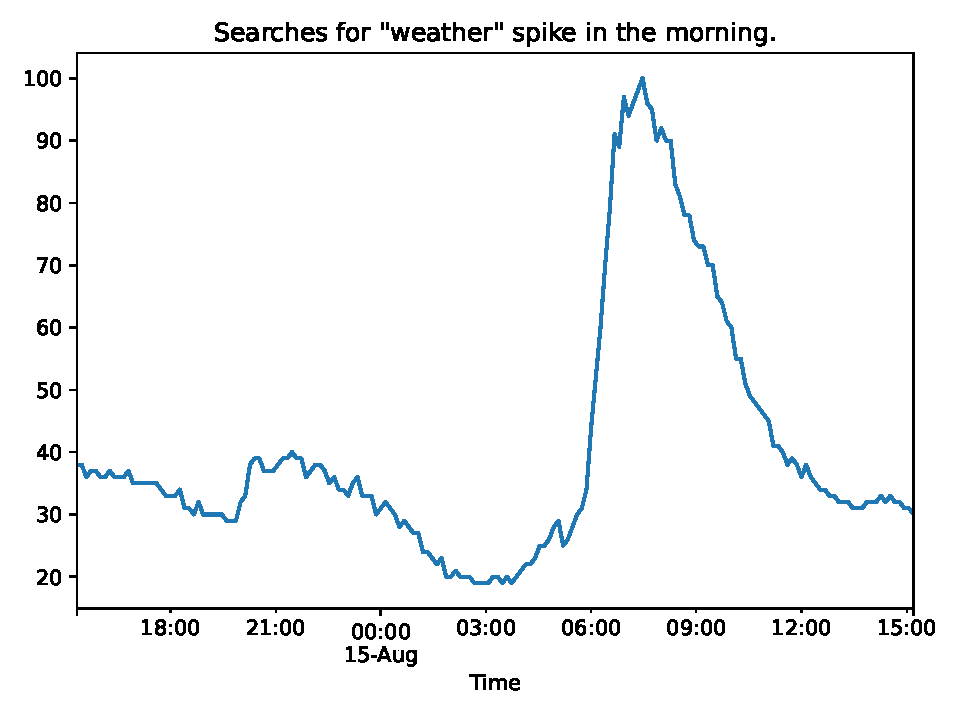
\includegraphics[width = .7\textwidth]{figures/proseplots/pd-dates.pdf}
\end{center}

Before we try to improve the formatting, see what happens if we try to use the axes plot method. 

\pyfile{ax-dates.py}

\begin{center}
    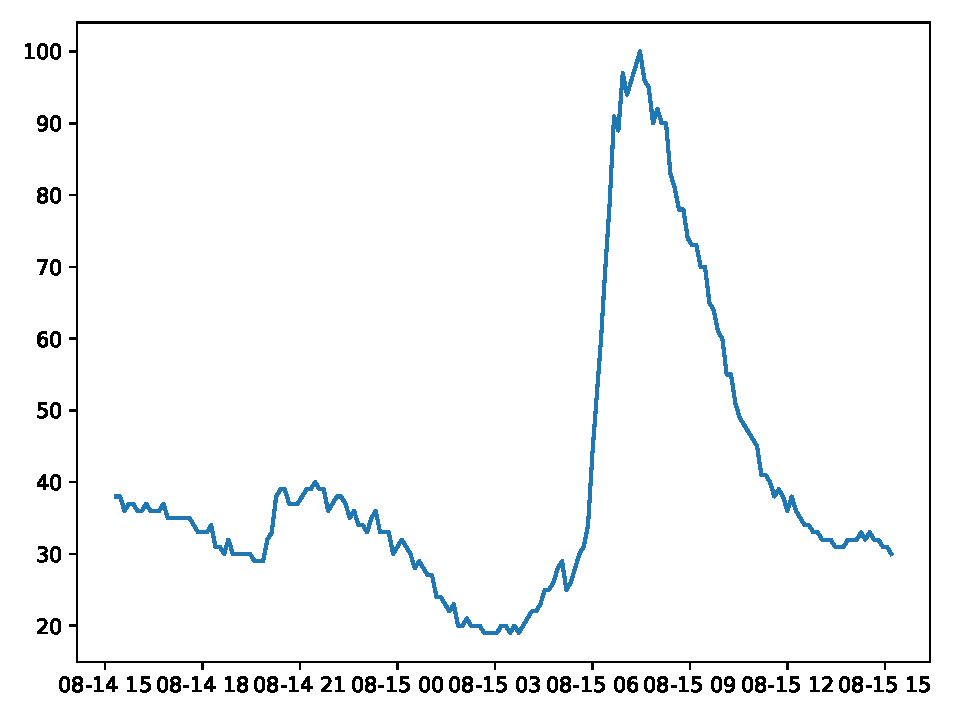
\includegraphics[width = .7\textwidth]{figures/proseplots/ax-dates.pdf}
\end{center}

You might find code using \code{plot_date()}, which used to be used in place of \code{plot()}. This is no longer necessary.


\subsection{Time Zone Handling}

%\code{plot_date()} also plots the dates according to a default UTC timezone, sometimes converting dates given in a different timezone. This can be modified with the \code{tz} parameter, but this requires covering 


For a deeper knowledge, see the \code{datetime.tzinfo} class and the \code{pytz} library. TK

\section{Ticks and Formatting}

\subsection{Date Formats}

The specific format of the displayed dates and times can be modified with \code{mdates.DateFormatter()}. This takes a format string and creates a formatter that can be passed to an axis method \code{set_major_formatter()} or \code{set_minor_formatter()}. 

Here are some common format codes, applied to Sunday January 30, 2000, 11:59PM, local to Louisville, Kentucky. These can all be verified with \code{pd.Timestamp(year = 2000, month = 1, day = 30, hour = 23, minute = 59, tz = 'America/Kentucky/Louisville').strftime()}.

\begin{center}
\begin{small}
{\setlength{\tabcolsep}{2em}
\begin{tabular}{ll}
\toprule
Code & Output/Example \\
\midrule
\code{'\%Y'} & 4-Digit Year \\
\code{'\%m'} & Month Number \\
\code{'\%d'} & Day of Month \\
\code{'\%B'} & Month Name \\
\code{'\%H'} & 24-Hour Clock Hour \\
\code{'\%M'} & Minute \\
\code{'\%H'} & 12-Hour Clock Hour \\
\code{'\%p'} & AM or PM \\
\code{'\%A'} & Day of Week \\
\code{'\%Z'} & Timezone Name \\
\code{'\%Y-\%m'} &   \code{'2000-01'}\\
\code{'\%Y\/\%m/\%d'} & \code{'2000/01/30'}\\
\code{'\%B \%y'} & \code{'January 00'}\\
\code{'\%H:\%M \%Z'} & \code{'23:59 EST'} \\
\code{'\%A \%I\%p'} & \code{'Sunday 11PM'}\\
\bottomrule
\end{tabular}}
\end{small}
\end{center}

A more complete list of format codes can be found at \link{https://strftime.org}{strftime.org}. Codes that generate actual names, like \code{'\%A'} or \code{'\%B'}, can be made lowercase to produce an abbreviated name. Notice that these formats create zero-padded numbers like \code{'07'} instead of \code{'7'}. On Mac or Linux, padding can be eliminated with the \code{'-'} modifier, using \code{'\%-H'} or \code{'\%-m'}
instead of \code{'\%H'} or \code{'\%m'} for example. On Windows, use \code{'#'}.

\pyfile{date-fmt.py}

\begin{center}
    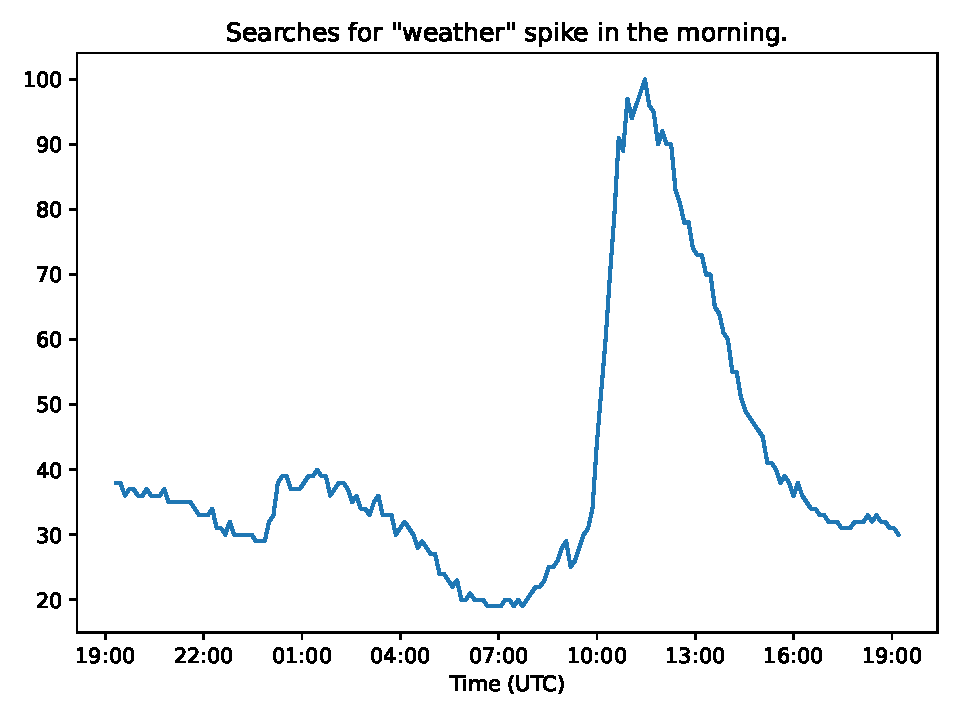
\includegraphics[width = .7\textwidth]{figures/proseplots/date-fmt.pdf}
\end{center}

\pyfile{date-fmt2.py}

\begin{center}
    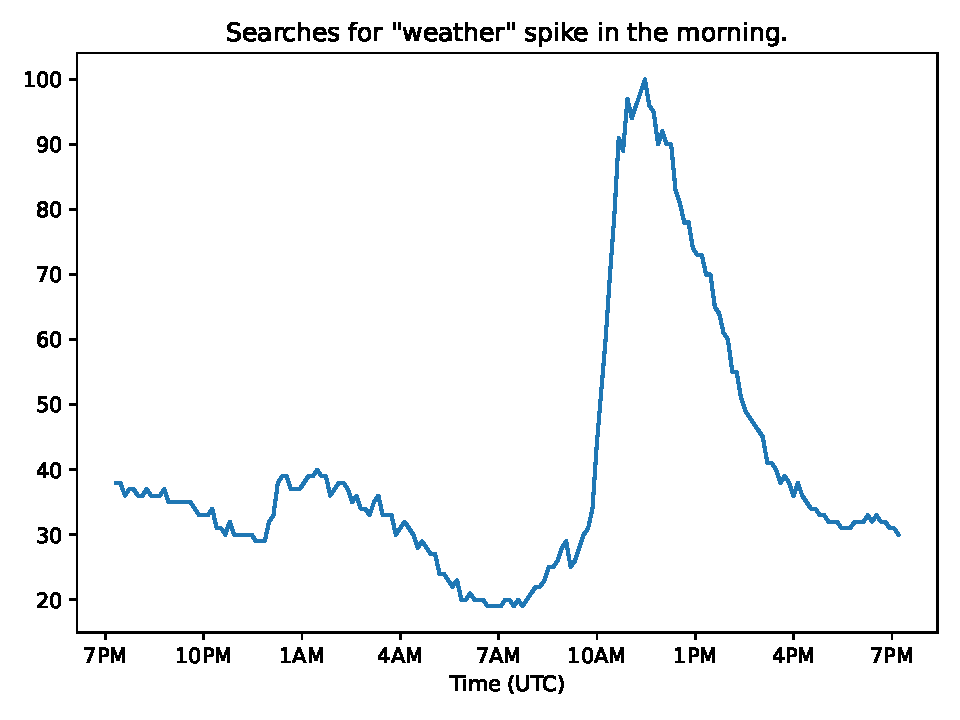
\includegraphics[width = .7\textwidth]{figures/proseplots/date-fmt2.pdf}
\end{center}
